\documentclass[11pt,compress,t,notes=noshow, aspectratio=169, xcolor=table, usenames,dvipsnames]{beamer}

\usepackage{../../style/lmu-lecture}
% Defines macros and environments
% This file is included in slides and exercises

% Rarely used fontstyle for R packages, used only in 
% - forests/slides-forests-benchmark.tex
% - exercises/single-exercises/methods_l_1.Rnw
% - slides/cart/attic/slides_extra_trees.Rnw
\newcommand{\pkg}[1]{{\fontseries{b}\selectfont #1}}

% Spacing helpers, used often (mostly in exercises for \dlz)
\newcommand{\lz}{\vspace{0.5cm}} % vertical space (used often in slides)
\newcommand{\dlz}{\vspace{1cm}}  % double vertical space (used often in exercises, never in slides)
\newcommand{\oneliner}[1] % Oneliner for important statements, used e.g. in iml, algods
{\begin{block}{}\begin{center}\begin{Large}#1\end{Large}\end{center}\end{block}}

% Don't know if this is used or needed, remove?
% textcolor that works in mathmode
% https://tex.stackexchange.com/a/261480
% Used e.g. in forests/slides-forests-bagging.tex
% [...] \textcolor{blue}{\tfrac{1}{M}\sum^M_{m} [...]
% \makeatletter
% \renewcommand*{\@textcolor}[3]{%
%   \protect\leavevmode
%   \begingroup
%     \color#1{#2}#3%
%   \endgroup
% }
% \makeatother


\title{Interpretable Machine Learning}
% \author{LMU}
%\institute{\href{https://compstat-lmu.github.io/lecture_iml/}{compstat-lmu.github.io/lecture\_iml}}
\date{}

\begin{document}


% Set style/preamble.Rnw as parent.

% Load all R packages and set up knitr

% This file loads R packages, configures knitr options and sets preamble.Rnw as
% parent file
% IF YOU MODIFY THIS, PLZ ALSO MODIFY setup.Rmd ACCORDINGLY...

% Defines macros and environments

 \newcommand{\titlefigure}{figure/counterfactuals_obj}
\newcommand{\learninggoals}{
\item Understand the motivation behind CEs
\item See the mathematical foundation of CEs}

\lecturechapter{Counterfactual Explanations}
\lecture{Interpretable Machine Learning}

% ------------------------------------------------------------------------------

\begin{frame}[c]{Example: Credit Risk Application}
	\begin{itemize}
		\item $\textbf{x}$: customer and credit information
		\item $y$: grant or reject credit
	\end{itemize}
	\begin{center}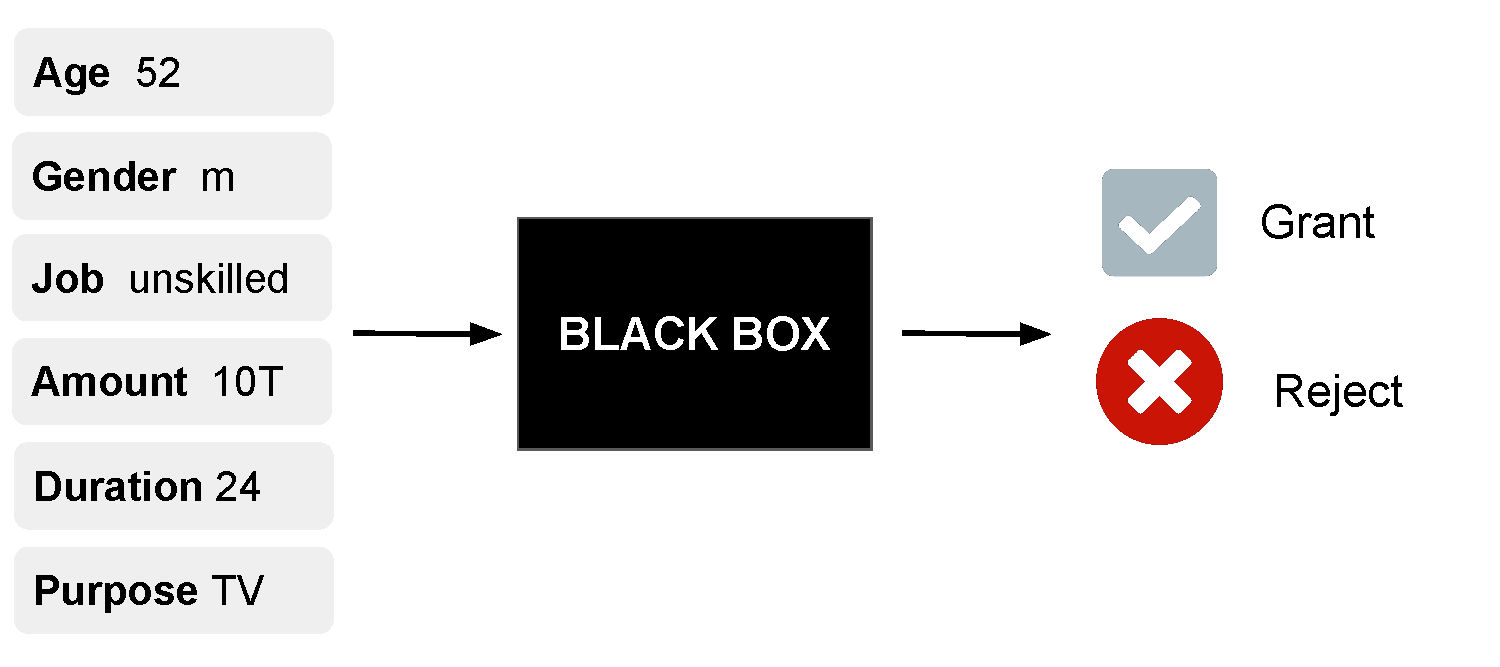
\includegraphics[width=0.6\linewidth, page=1]{figure/counterfactuals_credit.pdf} \end{center}

	Questions:
	\begin{itemize}
		\item Why was the credit rejected?
		\item Is it a fair decision?
		\item \textbf{How should $\xv$ be changed so that the credit is accepted?}
	\end{itemize}
\end{frame}


\begin{frame}[c]{Example: Credit Risk Application}
	Counterfactual Explanations provide answers in the form of "What-If"-scenarios.
	\begin{center}\includegraphics[width=0.6\linewidth, page=2]{figure/counterfactuals_credit.pdf} \end{center}

	``If the person was more skilled and the credit amount had been reduced to \$8.000,\\ the credit would have been granted."  \\[0.2cm]

\end{frame}


\begin{frame}[c]{Counterfactual Explanations: Main Idea}
	\begin{itemize}[<+->]
	    \item Counterfactual explanations == counterfactuals == CEs
	    \item Explain particular predictions of an ML model by presenting an alternative input whose prediction equals a desired outcome
		\item Represent \textbf{close neighbors} of a data point we are interested in,\\ but belonging to the \textbf{desired outcome}
		\item Reveal which minimal changes to the input are sufficient to receive a different outcome\\
		$\leadsto$ Useful if there is a chance to change the input features (e.g., by changing behaviour)
		\item The targeted audience of CEs are often end-users%, not ML engineers
	\end{itemize}
\end{frame}


\begin{frame}[c]{Aims \& Roles}
	CEs can serve various purposes, the user can decide what to learn from them.
	For example:  \\[0.2cm]
	``If the person had been \textbf{one year older} and the \textbf{credit amount had been increased} to \$12.000,\\ the credit would have been granted."  \\[0.2cm]
	\pause
	\begin{itemize}[<+->]
		\itemsep1.2em
		\item \textbf{Guidance for future actions:}\\ \textit{Ok, I will apply again next year for the higher amount.}
		\item \textbf{Provide reasons:}\\ \textit{Interesting, I did not know that age plays a role in loan applications.}
		\item \textbf{Provide grounds to contest the decision:}\\ \textit{How dare you, I do not want to be discriminated for my age in an application.}
		\item \textbf{Detect model biases:}\\ \textit{There is a bug, an increase in amount should not increase approval rates.}
	\end{itemize}
\end{frame}


\begin{frame}{Philosophical Basis}
%Interestingly, counterfactuals have a long-standing tradition in philosophy and, in fact the IML discussion of CEs is based on the work of Lewis (1973).
Counterfactuals have a long-standing tradition in analytic philosophy\\
$\leadsto$ %and, in fact the IML discussion of CEs is based on the work of Lewis (1973).
Accoding to \citebutton{Lewis (1973)}{https://doi.org/10.2307/2273738}, a \textbf{counterfactual conditional} is a statement of the form:

\begin{center}
``If $S$ was the case, $Q$ would have been the case."
		%\label{eq:sent}
\end{center}

\pause

	\begin{itemize}[<+->]
		\item $S$ is an event that must relate to a past event that didn't occur\\ $\leadsto$ counterfactuals run \textbf{contrary} to the \textbf{facts}
		\item Above statement is true, if in all possible worlds most similar to the actual world where $S$ had been the case, $Q$ would have been the case
		\item A world is similar to another if laws are maximally preserved between the worlds and only a few facts are changed
%		\item Lewis's proposal is hotly debated in philosophy, particularly his notion of similarity between worlds remains controversial.
	\end{itemize}
\end{frame}

\begin{frame}{Philosophical Basis}
% According to Lewis:\newline
%``$Q$ causally depends on $S$ iff, if $S$ were not the case $Q$ would not have been the case.''
	\begin{itemize}[<+->]
	\item Counterfactuals have largely been studied to explain causal dependence
		\item Causal dependence underlies the explanatory power\\
		$\leadsto$ good CEs point to critical causal factors that drove the algorithmic decision
		\item If maximal closeness is relaxed, causally irrelevant factors can become part of the explanation\\
		$\leadsto$ e.g., decreasing loan amount by \$20.000 and being one year older is recommended by the explainer although only loan amount might be causally relevant
		%Think of a case when a decrease in amount by \$20.000 and being one year older is recommended by the explainer to receive the loan while changing only the former suffices
		\item CEs are often contrastive, i.e., they explain a decision by referring to an alternative outcome\\
		$\leadsto$ e.g., if the loan applicant was 30 instead of 60 years old, the approved loan would have been over \$100.000 instead of \$40.000%This is also the reason why counterfactuals must be maximally close to initial inputs, otherwise changes are only sufficient but some of them might be unnecessary.
%		\item Current research on causality is based on Pearl's (2009) causal graphs. Instead of defining causality in terms of counterfactuals, Pearl's approach turns the story around and necessitates a representation of causal mechanisms to define CEs.
	\end{itemize}
%\footnote[frame]{Lewis, David (1973). Counterfactuals. Cambridge, MA: Harvard University Press. ISBN 9780631224952. }
\end{frame}

%\begin{frame}{Philosophical Basis: CEs as Contrastive}
%CEs are or can be easily translated into contrastive explanations and often vice versa. Contrastive explanations are answers to a question of the form ``why did Q' occur instead of Q?''.
%	\begin{itemize}
%	    \item  Contrastive explanations answer these questions by \textbf{contrasting} the actual scenario with a different scenario $S$ in which $Q$ had occurred.
%		\item According to psychologists [Miller (2019)], contrastive explanations are the gold standard of explanations in human-to-human interaction.
%		\item A CE becomes contrastive if its antecedent $S$ is presented in contrast to the actual scenario.
%	\end{itemize}
%\end{frame}

\begin{frame}{Mathematical Perspective}
	Terminology:
	\begin{itemize}
		\item $\xv$: original/factual datapoint whose prediction we want to explain
		\item $y' \subset \R^g$: desired prediction ($y' = 1000$ or $y' =$ ``grant credit") or interval ($y' = [1000, \infty[$)
	\end{itemize}
	\lz\pause
	A \textbf{valid} counterfactual $\xv'$ is a datapoint:
	\begin{enumerate}
		\item whose prediction $\fh(\xv')$ is equal to the desired prediction $y'$
		\item that is maximally close to the original datapoint $\xv$
	\end{enumerate}
	\lz\pause
	Reformulate these two objectives (denoted by $o_1$ and $o_2$) as optimization problem:
	
$$\argmin_{\xv'} \lambda_1 o_p(\fh(\xv'), y') + \lambda_2 o_f(\xv', \xv)$$

	\begin{itemize}
		\item $\lambda_1$ and $\lambda_2$ balance the two objectives
		\item Choice of $o_p$ (distance on prediction space) and of $o_f$ (distance on feature space) is crucial
	\end{itemize}
\end{frame}


\begin{frame}{Mathematical Perspective \citebutton{Dandl et al. (2020)}{https://arxiv.org/abs/2004.11165}}
	
	\begin{itemize}
		\item Regression: $o_p$ could be the L$_1$-distance $o_p(\fh(\xv'), y') = |\fh(\xv')-y'|$
		\item Classification:
		L$_1$-distance for scores and 0-1 Loss for labels, e.g., $o_p(\fh(\xv'), y') = \ind_{\{ \fh(\xv') \neq y' \}}$
		\pause
		\item $o_f$ could be the Gower distance (suitable for mixed feature space):
		$$o_f(\xv', \xv) = \Gower(\xv', \xv) = \frac{1}{p}\sum_{j = 1}^{p} \delta_G(x'_j, x_j)	\in [0, 1]$$
		The value of $\delta_G$ depends on the feature type (numerical or categorical):
		\begin{equation*}
		\delta_G(x'_j, x_j) =
		\begin{cases}
		\frac{1}{\widehat{R}_j}|x_j'- x_j| & \text{if $x_j$ is numerical} \\
		\ind_{\{ x_j' \neq x_j \}} & \text{if $x_j$ is categorical}
		\end{cases}
		\end{equation*}
		with $\widehat{R}_j$ as the value range of feature $j$ in the training dataset (to ensure that $\delta_G(x'_j, x_j)	\in [0, 1]$)
	\end{itemize}
%\footnote[frame]{Dandl S., Molnar C., Binder M., Bischl B. (2020) Multi-Objective Counterfactual Explanations. In: Bäck T. et al. (eds) Parallel Problem Solving from Nature – PPSN XVI. PPSN 2020. Lecture Notes in Computer Science, vol 12269. Springer, Cham.}
%\footnote[frame]{Verma et al. (2020). \href{https://arxiv.org/pdf/2010.10596.pdf}{Counterfactual Explanations for Machine Learning: A Review.}}
\end{frame}

\begin{frame}{Further Objectives}
	%While validity is a necessary condition for counterfactuals,
	Additional constraints can improve the explanation quality of the corresponding CEs\\
	$\leadsto$ popular constraints include sparsity and plausibility
	
	\lz

	\textbf{Sparsity:}
	\begin{itemize}[<+->]
		\item End-users often prefer short over long explanations\\
		$\leadsto$ %changes made to obtain
		counterfactuals should be \textbf{sparse} %(i.e., only few feature values should change)
		\item Objective $o_f$ can take the number of changed features into account (but does not have to)\\
		$\leadsto$ e.g., the L$_0$- and the L$_1$-norm (similar to LASSO) can do this
%		\item There could be a trade-off between the number of features changed and the total amount of change made to obtain a certain prediction.
        \item Independently from $o_f$, sparsity in the changes can be additionally considered by another objective that counts the number of changed features via the L0-norm:
        %we can also account for sparsity by adding an extra term to our objective that counts the number of changed features via the L0-norm
        $$o_s(\xv', \xv) = \sum_{j = 1}^p {\ind}_{\{ x'_j \neq x_j \}}$$
	\end{itemize}
\end{frame}

\begin{frame}{Further Objectives}
		\textbf{Plausibility:}
		\begin{itemize}
			%\item CEs should suggest alternatives that are plausible -- e.g, it is a bad idea to suggest a loan applicant to raise her income and get unemployed at the same time
			\item<1-> CEs should suggest plausible alternatives\\
			$\leadsto$ e.g., not plausible to suggest to raise your income and get unemployed at the same time
			\item<2-> CEs should be realistic and adhere to data manifold or originate from distribution of $\Xspace$\\
			$\leadsto$ avoid unrealistic combinations of feature values
			%We desire realistic CEs in the sense that they originate from the distribution of $\Xspace$ or adhere to the data manifold
			\item<3-> Estimating joint distribution of training data is complex, especially for mixed feature spaces\\
			$\leadsto$ Proxy: ensure that $\xv'$ is close to training data $\Xmat$
		\end{itemize}	
	\only<4>{
	\begin{columns}[c]
	\begin{column}{0.4\textwidth}
	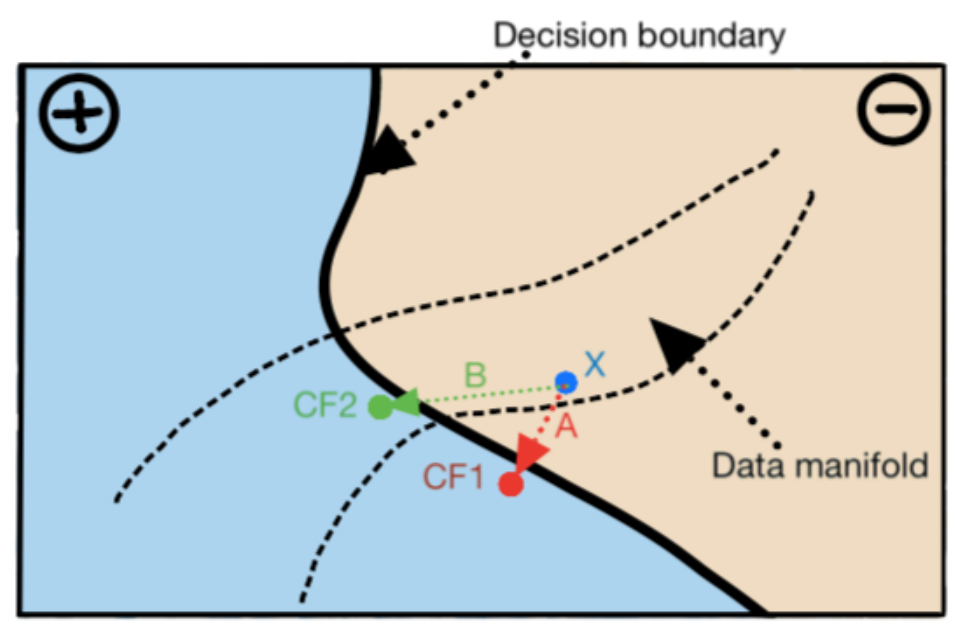
\includegraphics[width=1\textwidth]{figure/counterfactuals_obj}			
	\end{column}
	\begin{column}{0.6\textwidth}

\textbf{Example from \citebutton{Verma et al. (2020)}{https://arxiv.org/abs/2010.10596}} 
\begin{itemize}
    \item Two possible paths for \textcolor{blue}{$\xv$},			originally classified to $\pmb{\circleddash}$
    \item Two valid CEs in class $\pmb\oplus$: {\color{Red} CF1} and {\color{Green} CF2}
    \item {\color{Red} Path \textbf{A} for CF1} is shorter
    \item {\color{Green} Path \textbf{B} for CF2} is longer but adheres to data manifold
\end{itemize}
%Two possible paths for \textcolor{blue}{$\xv$},			originally classified in the negative class. The two counterfactuals (\textcolor{red}{CF1} and \textcolor{green}{CF2}) are valid. Note that the red path $A$ for CF1 is the shortest, whereas the green path $B$ for CF2 adheres closely to the manifold of the training data, but is longer.
\end{column}
\end{columns}
}
%\footnote[frame]{Verma et al. (2020). \href{https://arxiv.org/pdf/2010.10596.pdf}{Counterfactual Explanations for Machine Learning: A Review.}}

\end{frame}


\begin{frame}{Further Objectives}
	%\begin{itemize}
	%\item 
%For example, $o_4$ could then be the Gower distance of $\xv'$ to the nearest data point of the training dataset $\xv^{[1]}$

To ensure plausibility, $o_4$ could, e.g., be the Gower distance of $\xv'$ to its nearest data point of the training dataset which we denote $\xv^{[1]}$:
	
$$o_4(\xv', \Xmat) = \Gower(\xv', \xv^{[1]}) = \frac{1}{p} \sum_{j = 1}^{p}  \delta_G(x_j', x^{[1]}_j)$$
%\end{itemize}

We can extend the previous optimization problem by adding $o_s$ (for sparsity) and $o_4$ (for plausibility):

$$\argmin_{\xv'} \lambda_1 o_p(\fh(\xv'), y') + \lambda_2 o_f(\xv', \xv) + \lambda_3 o_s(\xv', \xv) + \lambda_4 o_4(\xv', \Xmat)$$

\end{frame}


\begin{frame}{Remarks: The Rashomon Effect}
%The solution to the optimization problem might not be unique, there can be many equally close inputs that obtain the desired classification. Correspondingly, there can be many different equally good explanations for the same decision. This is called the \textbf{Rashomon effect}.

\textbf{Issue (\textbf{Rashomon effect}):}
\begin{itemize}
    \item Solution to the optimization problem might not be unique
    \item Many equally close CE might exist that obtain the desired prediction\\
    $\Rightarrow$ Many different equally good explanations for the same decision exist
\end{itemize}

\lz\pause

\textbf{Possible solutions:}
	\begin{itemize}
	\item Present all CEs for a given $\xv$ (but: time and human processing capacity is limited)
		%\item We could present all CEs for a given case; however, time is limited and so is the human processing capacity
		%\item Another solution is to focus on one or few CEs; however, by which criterion should they be selected?
		\item Focus on one or few CEs (but: by which criterion should they be selected?)
	\end{itemize}
	
\lz\pause

\textbf{Note:}
	\begin{itemize}
        \item As the model is generally non-linear, inconsistent and diverse CEs can arise\\
        e.g. suggesting either an increase or decrease in credit duration (confuses the explainee)
		\item How to deal with the Rashomon effect is considered an open problem in IML
	\end{itemize}
\end{frame}

\begin{frame}[c]{Remarks: Model or Real-World}

	\begin{itemize}[<+->]
	\item Most CEs provide explanations of model predictions, but CEs might appear to explain the real-world for end-users\\
$\leadsto$ Transfer of model explanations to explain real-world is generally not permitted
	\item Consider a CE that proposes to increase the feature age by 5 to obtain the loan\\
	$\leadsto$ a loan applicant takes this information and applies 5 years later for the loan
	\item However, by then, many 
	%of their 
	other feature values 
	%properties 
	might have changed\\
	$\leadsto$ not only age, also other causally dependent features e.g. job status might have changed \\%after 5 years% since they are causally dependent on age like income or the job status
	$\leadsto$ \citebutton{Karimi et al. (2020)}{https://arxiv.org/abs/2002.06278} avoid this by considering causal dependencies between features
	\item Also, the bank's algorithm might change and previous CEs are not applicable anymore
	%\item Even worse, the user might have typos in the application and in fact no changes are necessary to obtain the loan.
%		\item Actionability: We could further strengthen above's plausibility criterion by requiring counterfactuals that do not change immutable features (e.g., race, city of birth, sex). Therefore, we could  search for counterfactuals only among a defined feasible set of counterfactuals $\mathcal{A}$.
%		\item Causality: We could also restrict the search to counterfactuals that maintain any known causal relations. In the real world, if one feature is changed it affects also other features. E.g., better skills lead to better salary, but also a higher age due to the necessary training.
	\end{itemize}
%\footnote[frame]{Karimi et al. (2021). Algorithmic Recourse: From Counterfactual Explanations to Interventions.  Proceedings of the 2021 ACM Conference on Fairness, Accountability, and Transparency. 353–362.}
\end{frame}


\endlecture
\end{document}
